A teleoperação do robô móvel Pioneer 3-AT foi a primeira parte do projeto desenvolvido. Essa etapa compreendeu o desenvolvimento de três subsistemas:

\begin{compactitem}
\item A comunicação do controle remoto Nintendo Wiimote com o computador mestre do ROS, \textit{framework} de robótica responsável pela integração de todo o sistema.
\item A escrita de um nó, denominação dos processos que rodam usando de funcionalidades do \textit{framework} ROS, para interpretar os comandos vindos do Wiimote e transformá-los em mensagens inteligíveis aos processos que controlam os atuadores do robô, transformando os comandos em ações no mundo real.
\item A escrita de um \textit{launcher} do ROS, arquivo XML que engloba todos os nós usados em um determinado sistema para atingir seus objetivos.
\end{compactitem}

A comunicação do Wiimote com o computador mestre do ROS foi feita usando do pacote \verb|wiimote| ~\cite{wiimote}. Esse pacote permite que, usando-se de comunicação \textit{bluetooth}, nós (\textit{nodes}) estabeleçam comunicação com o controle Wiimote através de tópicos. O pacote foi instalado no sistema fazendo-se \textit{download} do código a partir do repositório fornecido pelos autores ~\cite{gitwiimote} e compilando o mesmo.

A equipe instalou o pacote e conferiu as estruturas das mensagens geradas pelo mesmo, para que fosse possível utilizar com outros nós. Como a documentação não é muito clara, foram feitos testes para descobrir o mapeamento dos botões do controle. 

Entendido o funcionamento básico do pacote \verb|wiimote|, passou-se a desenvolver um nó (em C++), chamado de \verb|wii_oficinas_node| para gerenciar as mensagens do Wiimote, nó este que recebe as mensagens referentes ao estado atual do Wiimote e toma as ações adequadas de acordo com elas. A Figura~\ref{fig:wiimote_botoes} demonstra como os botões e os eixos do giroscópio integrado no Wiimote foram usados para controlar o robô móvel e o Kinect nele integrado. O fluxograma da Figura ~\ref{fig:wii_oficinas_node_flux} (no apêndice) descreve o funcionamento do nó \verb|wii_oficinas_node| e os fluxogramas da Figura ~\ref{fig:ints_wii} descrevem as rotinas de atendimento de interrupção para o nó.

\begin{figure}[H]
\centering
  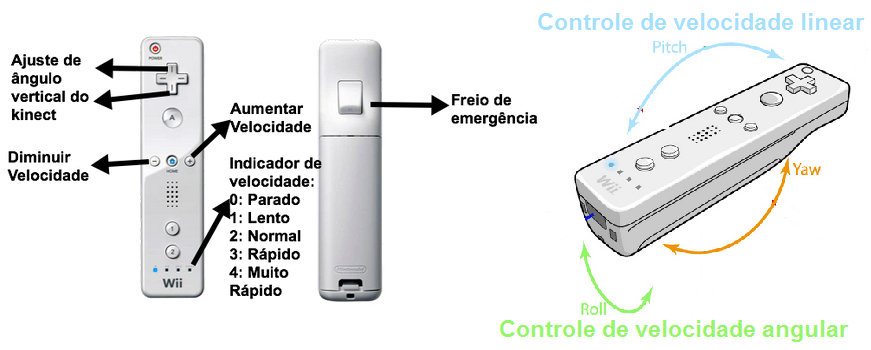
\includegraphics[width=12cm]{images/wiimote_botoes.png} 
\caption{\small{Representação gráfica do uso do controle remoto Nintendo Wiimote para teleoperação do robô móvel Pioneer 3-AT.}}
\label{fig:wiimote_botoes}
\end{figure} 

\begin{figure}[H]
\centering
  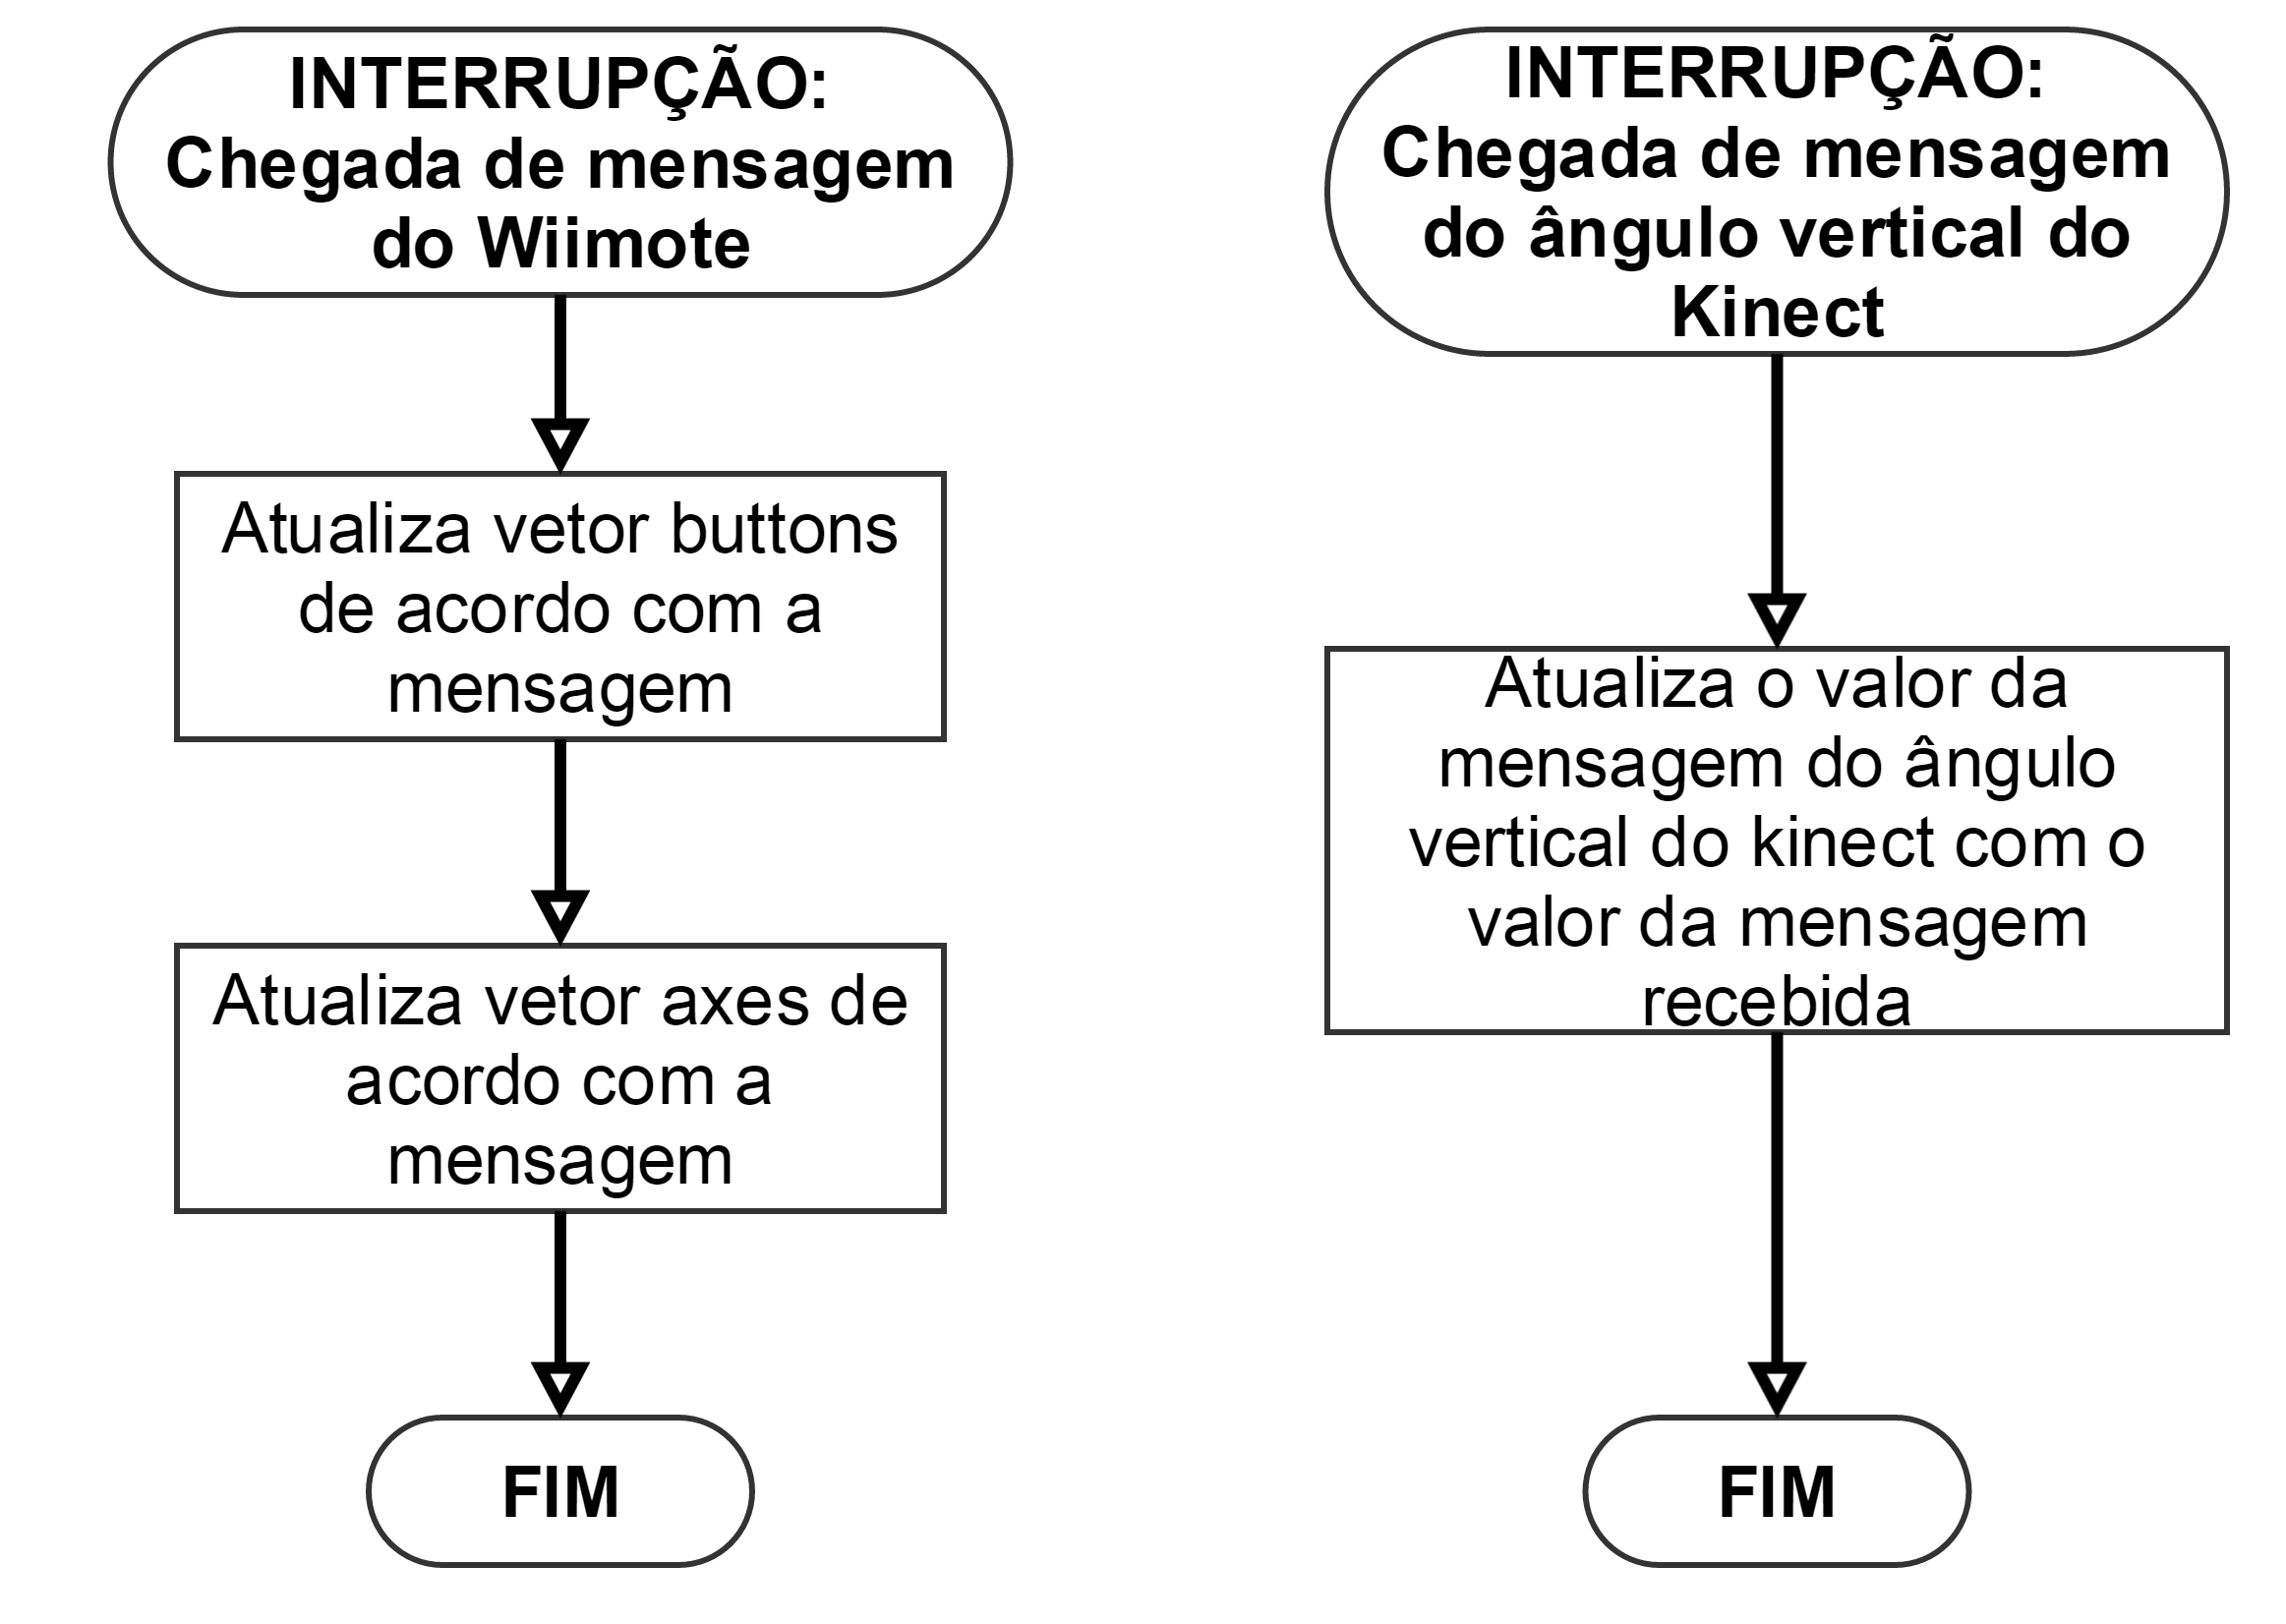
\includegraphics[width=12cm]{images/INTs.png} 
\caption{\small{Fluxograma representando as interrupções geradas pela chegada de mensagens e demonstrando como elas são tratadas.}}
\label{fig:ints_wii}
\end{figure}
